%*******************************************************************************
%****************************** Fourth Chapter *********************************
%*******************************************************************************

\chapter{LISP-Views: LISP mapping system monitor}
\label{cha:LISPViews}

% **************************** Define Graphics Path **************************
\ifpdf
    \graphicspath{{Chapter5/Pics/Raster/}{Chapter5/Pics/PDF/}{Chapter5/}}
\else
    \graphicspath{{Chapter5/Pics/Vector/}{Chapter5/}}
\fi

%-< ABSTRACT >--------------------------------------------------------------------
Proposed nearly ten years ago, LISP is still at an early stage. Currently only two experimental platforms have already been deployed in the Internet: LISP Beta Network and LISP-Lab. However, only the LISP Beta Network is monitored with LISPmon that partially monitors the mapping system once a day. To accompany the growth of LISP, a dynamic and complete monitoring system is required. Therefore, we propose LISP-Views, a dynamic versatile large scale LISP monitoring architecture. LISP-Views allows to automatically conduct comprehensive and objective measurements. After running LISP-Views in the wild for several months and comparing the monitoring results with LISPmon, we confirm that LISP-Views provides more detailed and accurate information. We observe the different behaviours between every network entity within mapping system, and also explore the current LISP performance for further improvements.

In the remainder, Sec.~\ref{sec:lispviews_archi_motivation} introduces the limitations of
LISPmon and why we propose a new LISP monitor. Sec.~\ref{sec:lispviews_archi_description} describes our proposed LISP monitoring architecture in details. Sec.~\ref{sec:lispviews_evaluation} validates LISP-Views by comparing with LISPmon. Sec.~\ref{sec:lispviews_results} provides the snapshot of what kind of further analysis can be done with our proposal. Finally, Sec.~\ref{sec:lispviews_conclusion} concludes the chapter. 
%-< ABSTRACT >--------------------------------------------------------------------


\section{Introduction}
\label{sec:lispviews_introduction}
% \begin{itemize}[noitemsep,topsep=0pt]
%     \item LISPmon is the only LISP monitor providing the basic LISP mapping information.
%     \item It cannot satisfy the more complex requirements and is not able to monitor the whole current LISP mapping system in real time.
%     \item LISP-Views is proposed.
%     \item LISP-Views provides more mapping information than LISPmon.
%     \item LISP-Views offers more specific information that LISPmon cannot provide.
% \end{itemize}
To promote the development of LISP and boost the related research, large scale flexible platforms are necessary. Two LISP-related platforms have been interconnected so far. The experimental LISP Beta Network testbed~\cite{lispbeta} is deployed since $2008$, and the LISP-Lab platform~\cite{lisplab} is open to external experimenters since $2015$. Currently, a unique LISP monitoring system called LISPmon~\cite{lispmon} supervises the global \acrshort{mds} and publishes the mapping information daily. However, it is known that the mapping information sometimes changes frequently within a day and that
the elements constituting the \acrshort{mds} are not always
consistent~\cite{yue2016stability}. We hence propose a dynamic versatile LISP
monitoring architecture, namely LISP-Views, to overcome these limitations. LISP-Views
automatically explores the whole \acrshort{mds} every 2 hours and stores the detailed
mapping information, so to facilitate the experimenters to evaluate the LISP
comprehensive performance.

We used a one-month long set of traces produced by LISP-Views to evaluate its performance and accuracy, including comparing it with LISPmon. We show that LISP-Views is more accurate than LISPmon since it monitors all the \acrshort{mds} elements in parallel. In addition, thanks to its detailed reporting, LISP-Views allows to assess high level metrics of LISP deployments such as reliability, latency, or configuration
issues.




%-< SECTION >--------------------------------------------------------------------
\section{Proposed Monitoring Architecture}
\label{sec:lispviews_archi}

%-< SUBSECTION >--------------------------------------------------------------------
\subsection{Motivation}
\label{sec:lispviews_archi_motivation}
% Limitations of LISPmon:
% \begin{itemize}[noitemsep,topsep=0pt]
%     \item Just monitors from one VP by querying one MR.
%     \item Once per day.
%     \item Has manual process upon MR issues.
%     \item Results are published as daily from beginning of 2010.
% \end{itemize}
% Thus, we propose a new versatile LISP monitoring architecture, called LISP-Views.

In order to move LISP forward, we need to deeply understand the behaviour of the different LISP network entities and since the \acrshort{mds} reflects the status of a LISP network as it stores all the mapping information, it is essential to be able to monitor the MDS. LISPmon was the first step towards a systematic LISP monitoring.  However, it monitors the \acrshort{mds} just from one vantage point (VP) once per day and only queries one MR.  Upon MR issues, LISPmon must be manually re-configured to  monitor another MR.  Yet the mapping information may be unstable and inconsistent between MRs, i.e., the mapping information sometimes dramatically changes within a day, and the Map-Replies from the different MRs may not coincide at a given time~\cite{yue2016stability}.  It is similar to the world-wide distributed BGP looking glass servers, which do not always provide the same responses for an IP address as the whole routing system may not have converged or because of routing policies. From such point of view, LISPmon has strong limitations since it is not able to detect the changes of mapping information within one day, and is not able to show the differences among MRs. Thus, we propose a new versatile LISP monitoring architecture, called LISP-Views, to monitor public LISP deployments, as well as to enable further performance evaluation of LISP defined by the users themselves. In fact, LISP-Views not only can be used to monitor LISP, but also can be used in the non-public networks, such as VxLAN~\cite{mahalingam2014virtual}.

LISP-Views is an open source implementation and has been designed to fulfill the following objectives:\footnote{Source code available on Github: \url{https://github.com/SeleneLI/LISP-Views}} 

\begin{enumerate}[noitemsep,topsep=0pt]
  \item LISP-Views queries to all the working MRs existing in current MDS, in
parallel, while LISPmon just queries one, aiming at building a complete view of
the current LISP status.
  \item LISP-Views periodically monitors all the MRs with arbitrary
  intervals,\footnote{This interval can be changed by the experimenters to accord
  their necessity. But in this chapter, the interval is set the shortest according to
  the process capacity of our server.} while LISPmon just does it daily, aiming
  at providing information about the mapping evolution at smaller time granularity.
  \item LISP-Views supervises the whole \acrshort{mds} without any manual process,
automatically reacting to failing components (e.g., unresponsive MRs).
  \item LISP-Views obtains the mapping information from all the MRs of the LISP
Beta Network as well as LISP-Lab platform, whereas LISPmon prefers to leverage the
MR of the former one.
  \item LISP-Views is flexible and configurable, with users able to define
different monitoring jobs and get the various measurements, whereas LISPmon
just publishes the mapping list daily.
  \item By design LISP-Views can be extended to be used as a monitoring facility for the internal deployed VxLAN.\footnote{In this chapter we focus on LISP.}
  \item LISP-Views is able to be deployed on multiple VPs over the world, while
  LISPmon publishes the results depending on one VP.
\end{enumerate}


%-< SUBSECTION >--------------------------------------------------------------------
\subsection{Description of LISP-Views}
\label{sec:lispviews_archi_description}
% LISP-Views consists of several modules with different functions. The detailed descriptions are as follows:
% \begin{itemize}[noitemsep,topsep=0pt]
%     \item Modules on a centralized server
%     \begin{itemize}[noitemsep,topsep=0pt]
%         \item Measurement 
%         \item Report
%         \item Raw Data
%     \end{itemize}
%     \item Modules deployed on several different \emph{VPs}
%     \begin{itemize}[noitemsep,topsep=0pt]
%         \item Crawler 
%         \item Sonar
%         \item Controller
%     \end{itemize}
% \end{itemize}

%-< FIGURE >--------------------------------------------------------------------
\begin{figure}[!t]
     \centering
     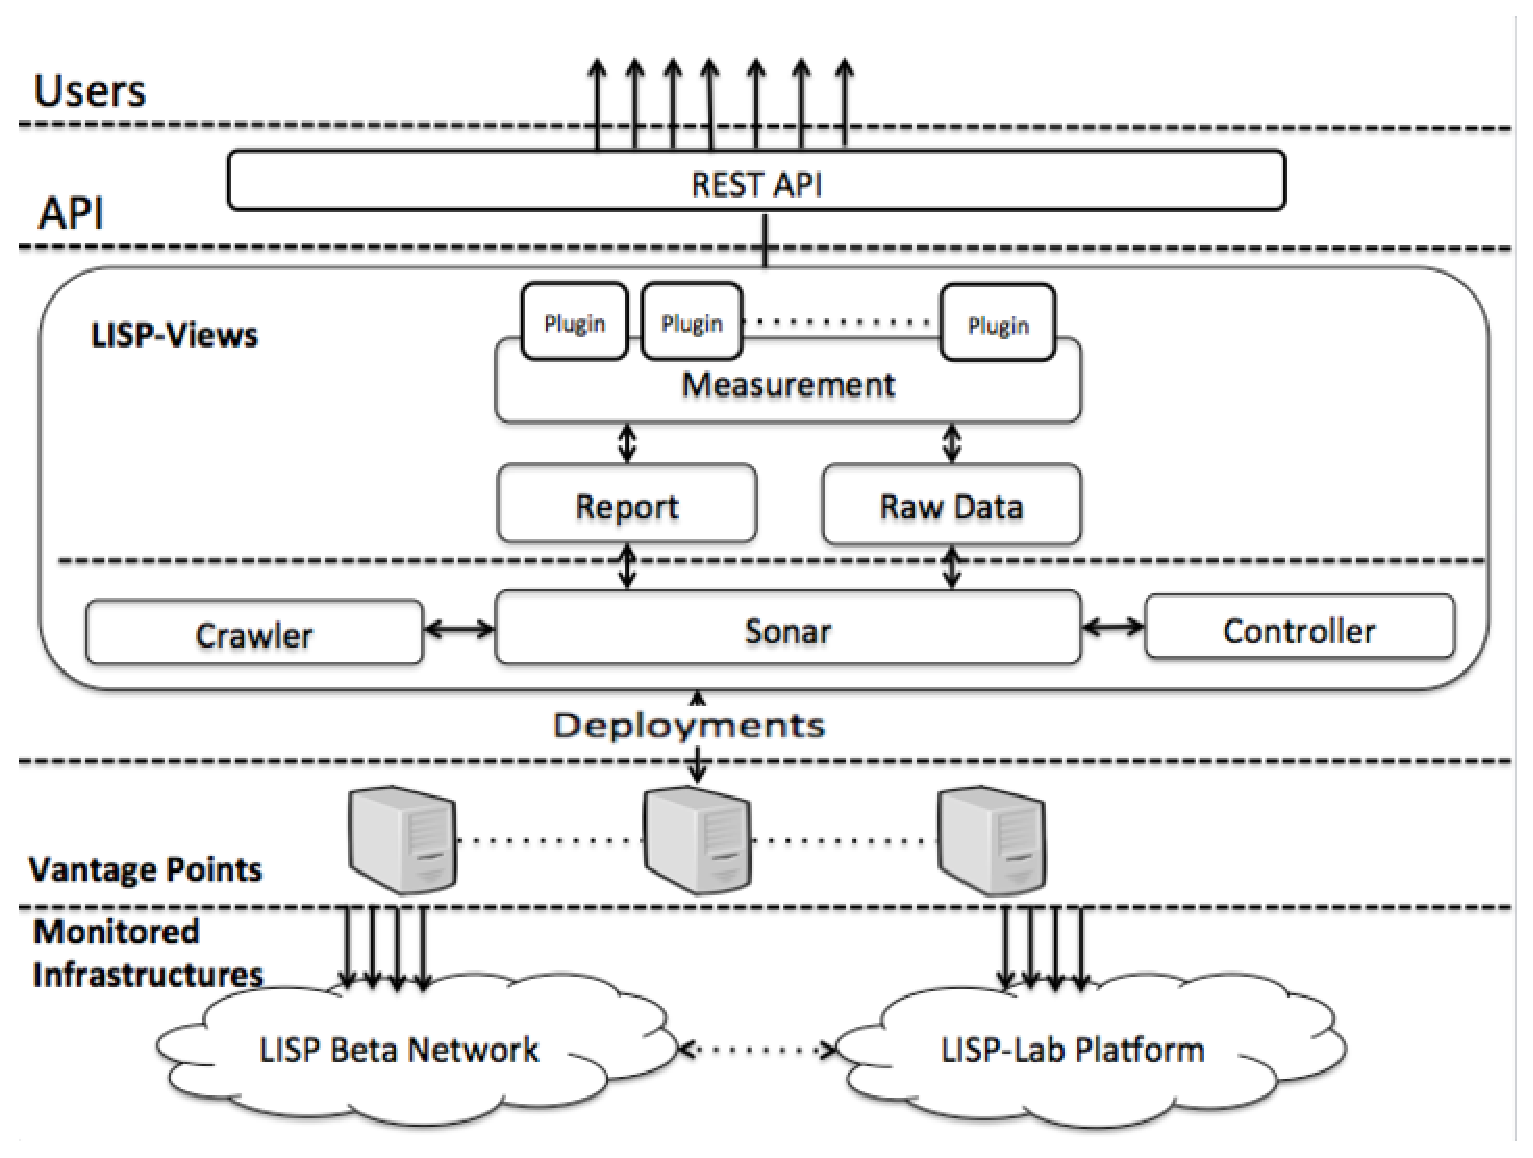
\includegraphics[width=0.9\textwidth]{Pics/LISP-Views_Arch.eps}
     \caption{Monitoring Architecture}
     \label{monitoring_arch}
\end{figure}
%-< END FIGURE >--------------------------------------------------------------------

The architecture of the proposed LISP-Views monitoring tools is depicted in Fig.~\ref{monitoring_arch}.  LISP-Views consists of several modules with different functions. The \emph{Measurement}, \emph{Report}, and \emph{Raw Data} modules are deployed on a centralized server while, the \emph{Crawler}, \emph{Sonar}, and \emph{Controller} modules can be deployed on several different \emph{VPs}.  As for now, LISP-Views is just deployed on one VP in Paris, France, where the monitor is developed and the centralized module is deployed. Nevertheless, we are planing to implement the distributed version of LISP-Views. For this reason, we will not discuss further how to deploy LISP-Views on multiple VPs. All the modules are implemented in \emph{Python} and described as follows:

\textbf{Sonar module}: the main module with two functions:
\begin{enumerate*}
   \item sending the LISP encapsulated Map-Requests and receiving the Map-Replies to/from all the existing MRs based on the standard~\cite{rfc6830};
   \item storing the received information in \emph{Report} and \emph{Raw Data} with different purposes.
\end{enumerate*}

The IP address that \emph{Sonar} uses to query to MRs is selected  either from the output of \emph{Crawler}, or from the recorded information in the previously produced \emph{Report}. The reasons are explained in the corresponding modules.

\textbf{Crawler module}: scans all the existing IPv4 addressing space using \emph{Sonar}.  If the queried IP (e.g., 192.0.2.1) has no Map-Reply, \emph{Crawler} increments the IP by one as the next queried IP (i.e., 192.0.2.2) and lets \emph{Sonar} send the Map-Request. If \emph{Sonar} obtains Negative or LISP Map-Reply, since the Reply contains a prefix (mentioned in Sec.~\ref{sec:background_lisp}), \emph{Crawler} sets the first IP beyond the returned prefix.  For instance if the returned prefix is 192.0.2.0/25, the next queried IP is 192.0.2.128.  Scanning the whole IPv4 address space takes very long time, and is mainly caused by time wasted waiting for no Map-Reply.  Indeed, no Map-Reply means to wait 3 seconds, and the next queried IP is just increased by one, instead of skipping a block of IP addresses like in the case of Negative/LISP Map-Reply.

\textbf{Report module}: contains the collected EID-prefixes in a list, as well as a list of MRs that answered. As crawling the address space may take long time but we aim to obtain the status of MRs as frequently as possible, \emph{Sonar} sends Map-Requests for the EIDs recorded in \emph{Report} only to MRs that have previously responded. Thus, it decreases the possibility to receive no Map-Reply, so that to get LISP status within a shorter time.

\textbf{Raw Data module}: contains all the detailed information of Map-Replies for each MR, such as Map-Reply type, RLOCs, required EID-Prefix, Round Trip Time (RTT) and the returned source for each round specify with $Time Stamp$ (regardless the source of \emph{Sonar}).  So, it can be used to perform thorough performance analysis of MDS. Moreover, since the \emph{Raw Data} is stored according to the MR, it is possible to track the performance of the MRs individually.

\textbf{Measurement module}: provides the composition of requested measurements (i.e., select different measurement plug-ins) based on the analysis of \emph{Raw Data} and \emph{Report}.

\textbf{REST API}: is connected to \emph{Measurement module} so that the users can launch a custom experiment by setting the experiment time, the monitored MRs, and obtain the different aspects of LISP status.  We are currently implementing the REST API, so for this paper the execution of measurements was performed using command lines.

\textbf{Controller module}: synchronizes all the modules in LISP-Views and also specifies the start and stop time of producing both \emph{Report} and \emph{Raw Data}. The interval of generating \emph{Report} and \emph{Raw Data} can be changed according to the hardware processing capability. However, since the inconsistency between MRs exits, the interval of producing Report and Raw Data for every MR differs from each other. Thus, the interval set in Control module should cover the slowest MR. 


%-< SECTION >--------------------------------------------------------------------
\section{LISP-Views Validation}
\label{sec:lispviews_evaluation}


%-< SUBSECTION >--------------------------------------------------------------------
\subsection{Methodology}
\label{sec:lispviews_evaluation_meth}
% \begin{itemize}[noitemsep,topsep=0pt]
%     \item Deployed LISP-Views on one VP, which is an xTR of LISP-Lab platform. 
%     \item Monitored during one month (from 0:00 September 4\textsuperscript{th} to midnight of October 4\textsuperscript{th} 2016).
%     \item The interval to produce \emph{Report} was 6 hours, and the interval to produce \emph{Raw Data} was 2 hours.
%     \item The analyzed results used in this chapter are collected from \emph{Raw Data} and \emph{Report}.
% \end{itemize}

In order to validate and evaluate the LISP-Views monitoring tool, we used raw data and report collected during one month (from 0:00 September 4\textsuperscript{th} to midnight of October 4\textsuperscript{th} 2016), by deploying LISP-Views on one VP, which is an \acrshort{xtr} of LISP-Lab platform.

The interval to produce reports was 6 hours, and the interval to produce raw data was 2 hours. Unfortunately, both MRs of LISP-Lab platform just responded to the Map-Requests at the first time and then stopped. They were not able to handle large number of queries, because the Map-Requests fill the request queues, which are not deployed in manner to sufficiently follow up the queries, resulting a drop in the MRs.  Per-se this is a success, because this bug was unknown, and the OpenLISP coders are working on a fix.  All the results of evaluation used in this section only depend on the 6 working MRs of LISP Beta Network (3 in Europe, 1 in US and 2 in Asia) and the other 6 MRs were down at the moment of conducting the experiment. The aim of the work is to validate LISP-Views by assessing if it provides at least the same results as LISPmon.


%-< SUBSECTION >--------------------------------------------------------------------
\subsection{LISP-Views vs. LISPmon}
\label{sec:lispviews_evaluation_com}
% The comparison between LISPmon and LISP-Views.
% \begin{itemize}[noitemsep,topsep=0pt]
%     \item In most cases, LISP-Views receives around 20 LISP Map-Replies more than LISPmon.
%     \item LISP-Views detects that there were issues to normally receive LISP status, whereas
% LISPmon hides the reality.
%     \item LISP-Views finds that the change of overall Map-Replies is mainly affected by LISP Map-Replies.
%     \item LISP-Views observes that MRs may not work normally in some rounds but they are able to recover fast.
% \end{itemize}

%-< FIGURE >--------------------------------------------------------------------
\begin{figure}[!t]
     \centering
     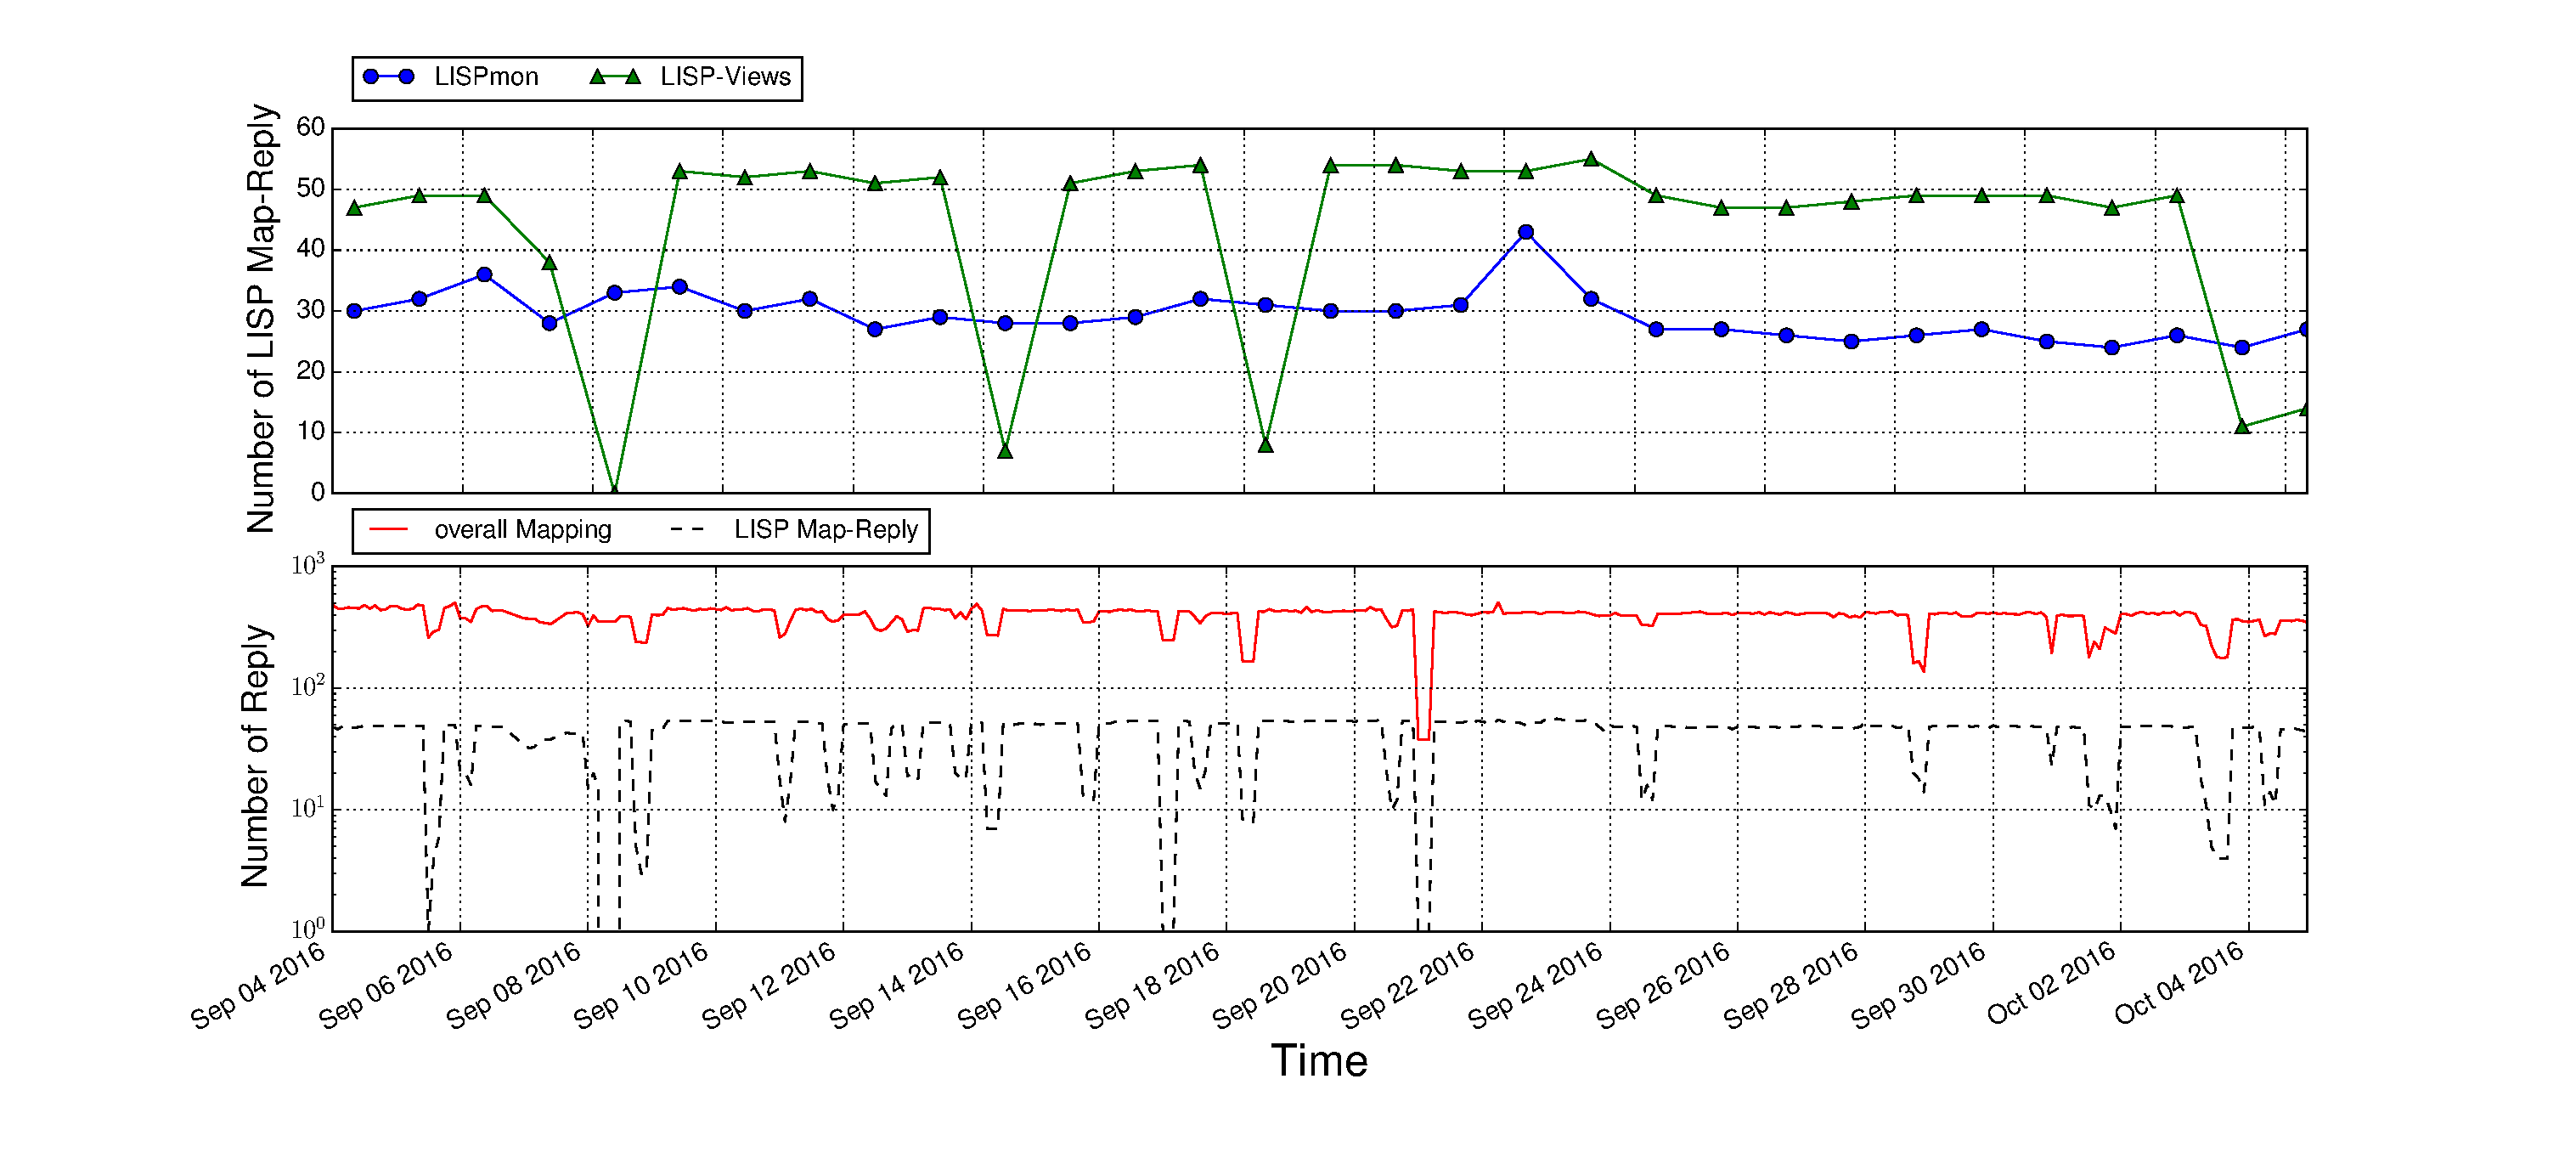
\includegraphics[width=1.1\textwidth]{Pics/LISPmon_comparison_all.eps}
     \caption{Comparison between LISPmon and LISP-Views. The upper
sub-figure shows the number of LISP Map-Reply from LISPmon generally at
7:00 and LISP-Views exactly at 8:00 over days. The bottom sub-figure
indicates the LISP Map-Reply and overall Mapping from LISP-Views over time with
an interval of 2 hours.}
     \label{lispmon_comparison}
\end{figure}
%-< END FIGURE >--------------------------------------------------------------------

In this section, we compare LISPmon and LISP-Views, so to asses if subset of information comparable between the two monitoring plateforms are identical, hence validating LISP-Views.  As we indicated in Sec.~\ref{sec:lispviews_archi_motivation}, at any time LISPmon just queries one MR, on LISP Beta Network once per day and generally begins at 7:00~a.m.. The queried MR is changed sometimes when it has issues. LISP-Views, however, keeps sending Map-Requests to all the 6 MRs with an interval of 2 hours everyday, so to retrieve the actual real status of each MR.

Fig.~\ref{lispmon_comparison} shows the number of LISP Map-Replies received from LISPmon and LISP-Views over time. The upper sub-figure makes a comparison between the 2 monitors. The line with point is obtained from the daily LISPmon publications, indicating the number of LISP Map-Replies returned by one MR in an uncertain time monitoring round every day. To facilitate the comparison, we pick up the results from LISP-Views aft 8:00 a.m., which is the nearest experimental round to LISPmon. As presented in the curve with triangle symbols, LISP-Views reflects the fact of a combination of the number of LISP Map-Reply containing the different EID-prefixes from all the MRs at a fixed experiment time. In most cases, LISP-Views receives around 20 LISP Map-Replies more than LISPmon, reflects the fact that the MRs are not coherent at any time due to the existence of convergence time for synchronizing the mapping information among them. The other 5 days, where LISP-Views receives very few LISP Map-Replies, show that there were issues to normally receive LISP status at that time, whereas LISPmon always presents a smoother trend but hides the reality.

The lack of stability can be better appreciated in the bottom sub-figure of Fig.~\ref{lispmon_comparison}. Such figure depicts the number of LISP Map-Reply (in dashed line) and the overall Mapping (LISP and Negative Map-Reply, in solid line) from LISP-Views for every 2 hours monitoring round during the whole experiment. Although the number of Map-Replies presented in the figure is still the combination of results from 6 MRs when the returned EID-prefixes are different, it shows that the MRs are not quite stable. Sometimes the MRs even provide 0 or less than 10 LISP Map-Replies, but in the next experiment round, the number is recovered. Besides, we evaluate the total number of successful queries every 2 hours. It also presents the behavior of instability, where it generally oscillates between 400 and 500, but it occasionally drops lower than 300. Both solid and dashed lines have almost same changing trend, indicating that the change of overall Map-Replies is mainly affected by LISP Map-Replies. Monitoring rounds where the number of LISP Map-Replies approaches 0 but where  Negative Map-Replies are still received indicate issues at the MRs, especially for answering the LISP Map-Reply.

%-< FIGURE >--------------------------------------------------------------------
\begin{figure}[!t]
        \centering
        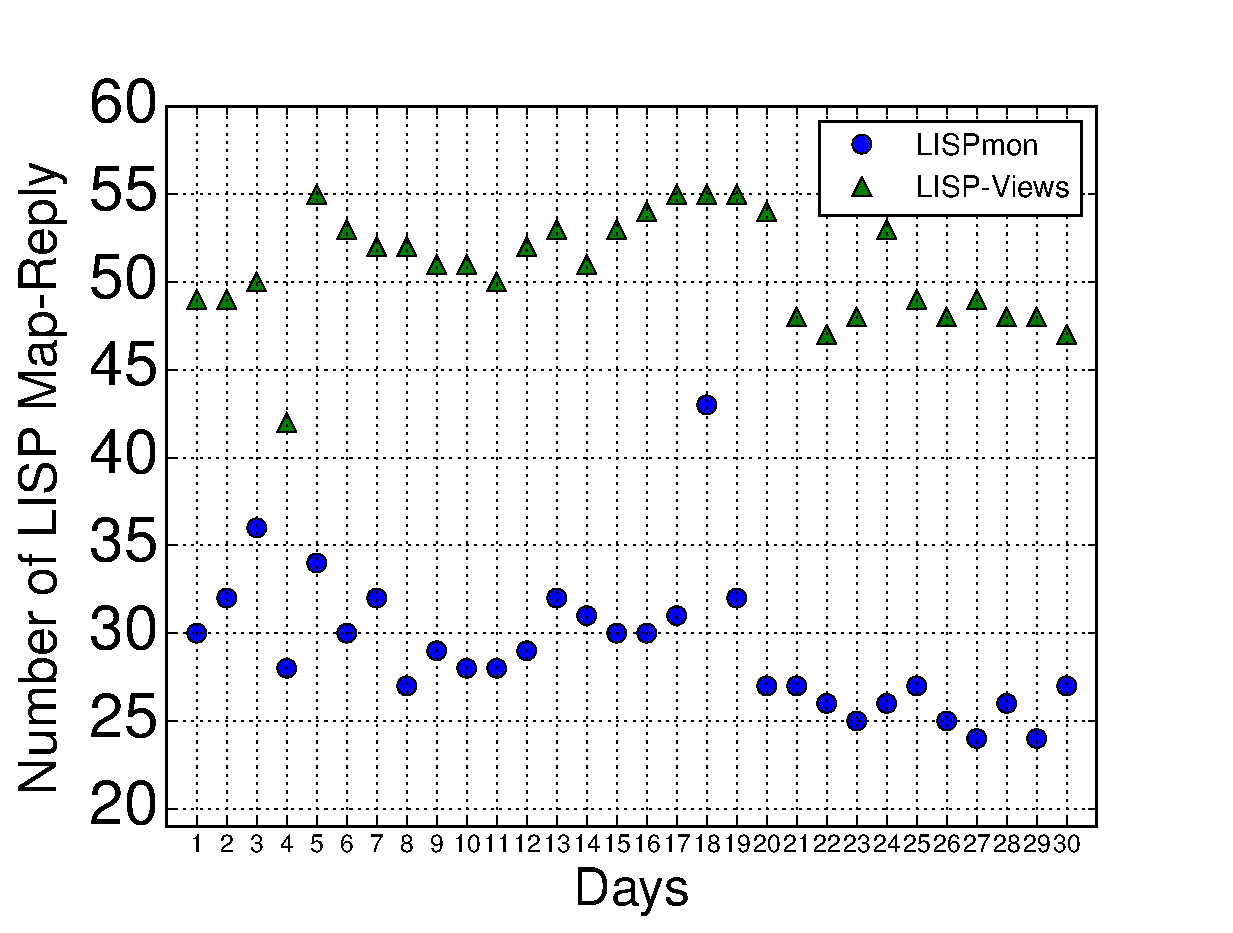
\includegraphics[width=0.8\textwidth]{Pics/LISPmon_comparison_day.eps}
        \caption{Comparison between the LISP Map-Reply of LISPmon and LISP-Views over days}
        \label{lispmon_comparison_day}
\end{figure}
%-< END FIGURE >--------------------------------------------------------------------

We compared the number of received LISP Map-Replies within a whole day between LISPmon and LISP-Views over 30 days. Shown in Fig.~\ref{lispmon_comparison_day}, as LISPmon only publishes one record each day, the number (blue points) is exactly identical to those in Fig.~\ref{lispmon_comparison}. LISP-Views, however, provides a combination of LISP Map-Replies not only from all MRs but also from 12 monitoring rounds within one day. We observe that our monitor architecture receives more LISP Map-Replies than LISPmon in all days with a large difference. 83.3\% of the time LISP-Views receives more than 20 LISP Map-Replies. The maximum number of LISP Map-Replies that our proposed monitor obtains is 55, while the maximum value for LISPmon is 43. Differently from the upper sub-figure of Fig.~\ref{lispmon_comparison}, where LISP-Views occasionally receives nearly 0 LISP Map-Replies, the total number within a whole day is always more than 40, which illustrates that the MRs may not work normally in some rounds but they are able to recover fast. 

Since LISP-Views repeats querying simultaneously to every MRs, it is able to report on the status of each MR at anytime. It provides more complete mapping information compared to LISPmon and is also able to highlight sporadic issues with MRs.


%-< SECTION >--------------------------------------------------------------------
\section{Dissecting LISP with LISP-Views}
\label{sec:lispviews_results}
% This section presents several examples of how LISP-Views can be used to dissect LISP and obtain in-depth
% results.
% \begin{itemize}[noitemsep,topsep=0pt]
%     \item Used the same dataset in Sec.~\ref{sec:evaluation_meth}.
%     \item Reliability of each MR is inconsistent.
%     \item RTTs for getting mapping information from each MR is different.
%     \item CDF of RTT comparison between LISP and Negative Map-Reply.
%     \item Percentage of mapping source.
%     \item CDF of the number of RLOCs.
%     \item Demonstrate an example about one type of measurement captured on LISP-Views website.
% \end{itemize}

After validating LISP-Views in the previous section, this section presents several examples of how LISP-Views can be used to dissect LISP and obtain in-depth results. The experimental dataset used is the one in Sec.~\ref{sec:lispviews_evaluation_meth}.
% The methodology used is exactly same to Sec.~\ref{sec:evaluation_meth}.

%-< FIGURE >--------------------------------------------------------------------
\begin{figure}[!t]
        \centering
        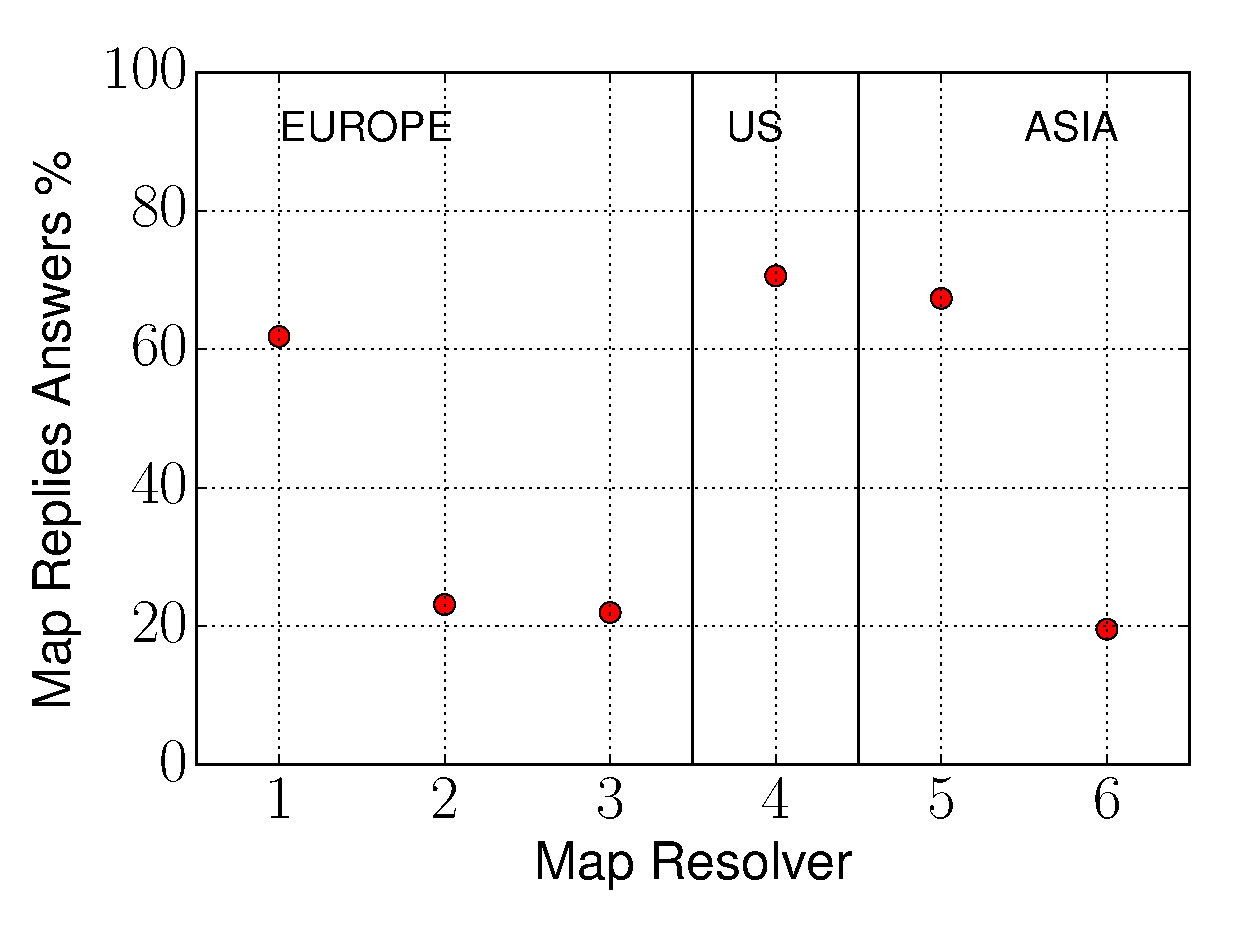
\includegraphics[width=0.8\textwidth]{Pics/Reliability.eps}
        \caption{Reliability of each MR}
        \label{MRs_reliability}
\end{figure}
%-< END FIGURE >--------------------------------------------------------------------
Fig.~\ref{MRs_reliability} shows the \emph{Reliability} of each MR during our
data collection, by calculating the percentage of successful queries over the
total number of Map-Requests. MR1, MR4, and MR5 give the highest
reliability values, which are more than 60\%. The lowest reliability values,
about 20\% are observed for MR2, MR3, and MR6. In general, the
reliability of each MR is different and low compared to the years of 2012 and
2013 presented in~\cite{coras2014performance}, which coincides with the fact
that there was a change of the MRs architecture on LISP Beta Network that year,
and an updated-software was tested on MRs as well.  The low value of
reliability is caused by MRs having an unstable behaviour, as shown in
Fig.~\ref{lispmon_comparison}, the number of Map-Reply changes heavily over
time, and especially the number of LISP Map-Reply sometimes drops to 0.

In order to understand the behavior of each MR in terms of latency, we analyze
the median RTT obtained from our dataset. The RTT here refers to the Round Trip
Time from sending out the Map-Request until receiving the Map-Reply.
Fig.~\ref{median_rtt_per_map-resolver} shows that the best performance come
from MR1, MR3, MR4, and MR5; since the overall RTTs are much lower than
the others.  For MR3, the number of LISP Map-Replies is much higher than the
number of Negative Map-Replies, probably because its embedded Map-Server
registers less EID-prefixes hence requiring Map-Requests to be forwarded to a
remote MS. Then, the Map-Request is forwarded to the \acrshort{xtr}, where the remote MS
registers and the \acrshort{xtr} gives back the Map-Reply. Compared to the Negative
Map-Replies, which are normally returned by MR, LISP Map-Replies take longer
time, especially in this case. However, MR2 and MR6 present very high
latency, particularly for MR2 (located in Europe), but its RTT is even higher
than MR5, which is located in Asia. It is mainly caused by a very high CPU
usage of these two MRs preventing them sometimes to reply.  If we focus on the
RTT of LISP Map-Replies, only MR1, MR4, and MR5 provide the best
behavior, which coincides with the result of Fig.~\ref{MRs_reliability} on
reliability. The high RTTs of LISP Map-Replies are from the other 3 MRs,
where the median RTT is around 1300 ms, is caused by the failed queries.
Furthermore, it also explains why we can always receive the Negative
Map-Replies, but the number of LISP Map-Replies is sometimes quite low in
Fig.~\ref{lispmon_comparison}. Half of LISP Map-Replies are more than 1300~ms
and partly even more than 3~s. Since our measurement timeout is set to 3~s
it implies that some Map-Replies are dropped by our measurement unit.  As the
RTT of Negative Map-Replies is generally lower, we can receive more of them. This
phenomenon may be very biased by the VP location. Thus, deploying LISP-Views on
multiple VPs to get more reliability information is a paramount future work. In
addition, Fig.~\ref{median_rtt_per_map-resolver} presents that the number of
Map-Replies returning from the MRs  located in Europe and US is indeed higher
than the number of Negative Map-Replies, which is expected. But both Asian MRs
return LISP Map-Replies faster than Negative Map-Replies. The reason of this 
observation is unclear and requires further exploration.
%-< FIGURE >--------------------------------------------------------------------
\begin{figure}[!t]
     \centering
     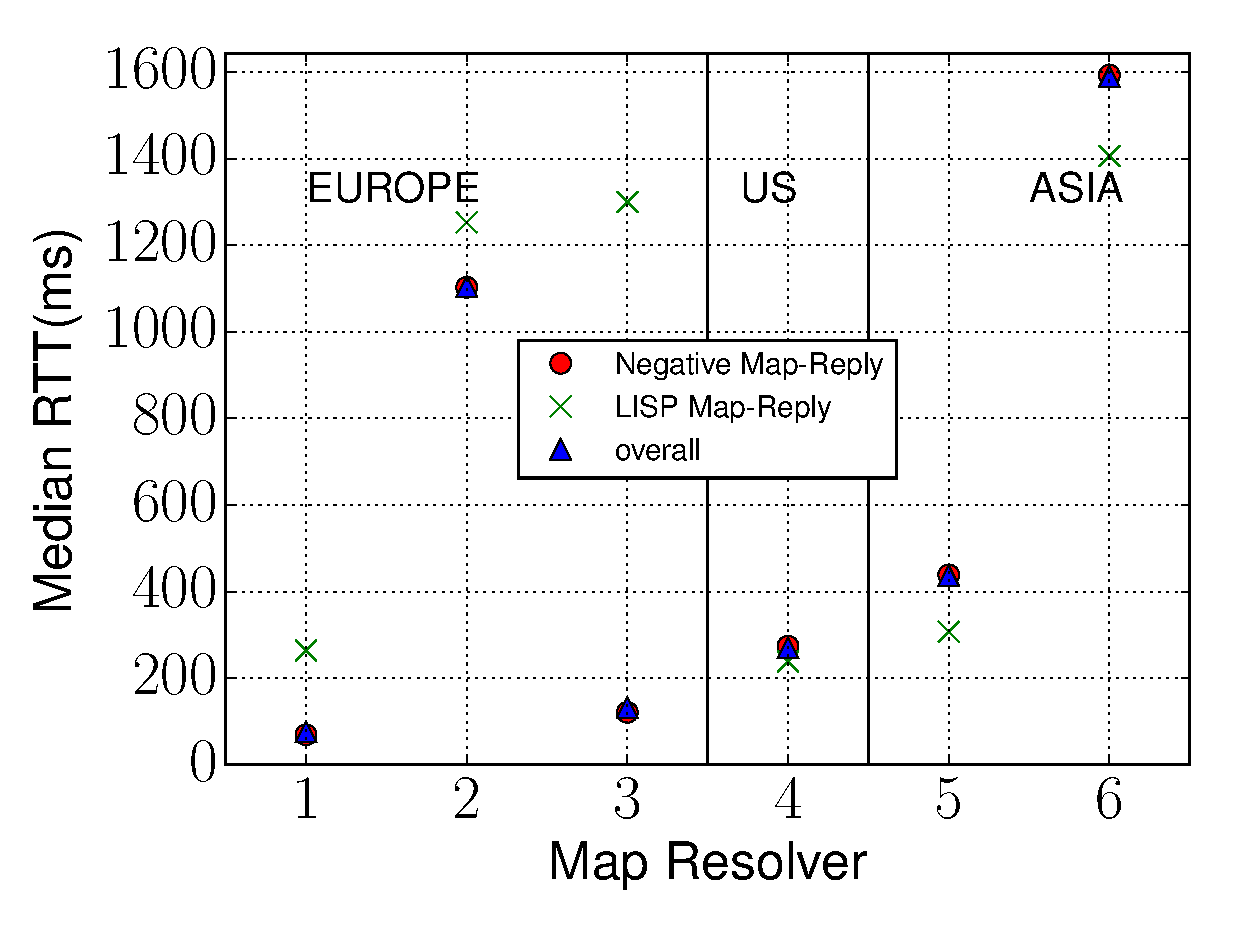
\includegraphics[width=0.8\textwidth]{Pics/median_of_RTT.eps}
     \caption{Median RTT per MR (In the most time, the Negative Map-Reply and overall are overlapped.)}
     \label{median_rtt_per_map-resolver}
\end{figure}

%-< FIGURE >--------------------------------------------------------------------
\begin{figure}[!t]
        \centering
        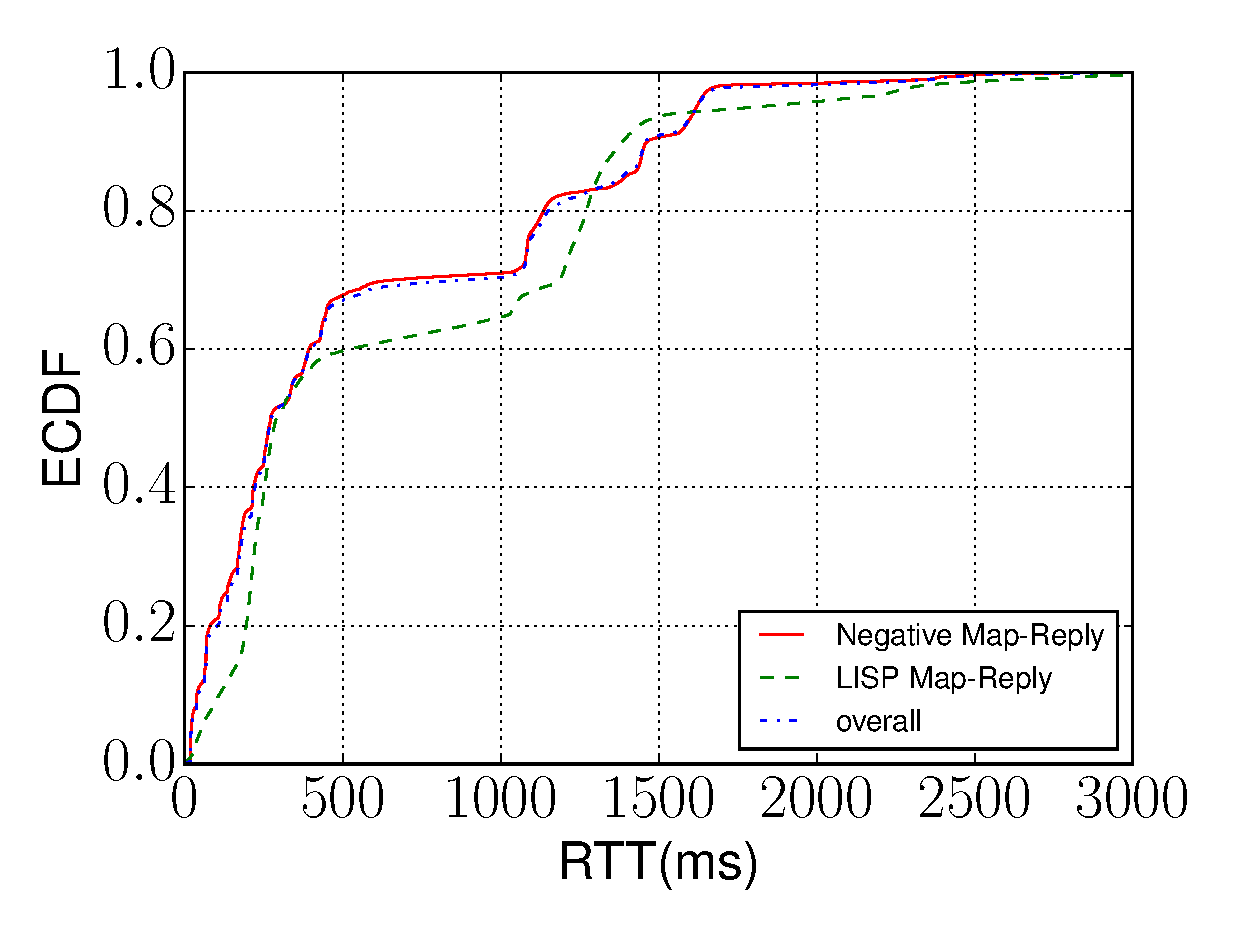
\includegraphics[width=0.8\textwidth]{Pics/ecdf_of_RTT.eps}
        \caption{ECDF RTT comparison between LISP and Negative Map-Reply}
        \label{ecdf_rtt_lisp_negative}
\end{figure}
%-< END FIGURE >--------------------------------------------------------------------
We also calculate the Empirical Cumulative Distribution Function (ECDF) of the
RTT for the 6 MRs. Fig.~\ref{ecdf_rtt_lisp_negative} provides the ECDF of the
RTT for Negative, LISP, and overall Map-Replies. As indicated in
Sec.~\ref{sec:background_lisp}, the LISP \acrshort{mds} needs more time to solve a
complete mapping (LISP Map-Reply) than the Negative Map-Reply.  We observe that
the Negative Map-Reply is indeed faster than the LISP Map-Reply until the RTT
reaches 1000 ms, then the behavior changes, i.e., the LISP Map-Reply
sometimes becomes faster. What's more, we find that 67.03\% of RTTs within
500 ms, 70.33\% less than 1000 ms and 90.88\% don't exceed 1500 ms
for overall Map-Replies. In details, for the Negative Map-Reply, we found that
67.8\% of RTT values within 500 ms, for the LISP Map-Reply that 59.7\% of
RTT values less than 500 ms. This figure almost presents a bi-modal
distribution, where 500 ms is a peak and 1300 ms is another one. These two
high occurrences of RTTs are exactly the most two frequent latency in
Fig.~\ref{median_rtt_per_map-resolver}.


%-< TABLE >--------------------------------------------------------------------
\begin{table}[!t]
    \centering
    \caption{Percentage of Mapping Source}% ~\akram{keep}
    \label{tab:percentage_of_received_from}{
	% \resizebox{0.9\textwidth}{!}{%
        \begin{tabular}{c|c|c|c}
            \hline\hline
                Map-Reply Type     & Map Resolver   & xTR       & Other \\ \hline
                Negative Map-Reply &  98.79\%       &  -        &  1.21\% \\ \hline
                LISP Map-Reply     & 0.14\%         & 88.37\%   &  11.49\%  \\ \hline\hline
        \end{tabular}
        }
\end{table}
%-< END TABLE >--------------------------------------------------------------------

The dataset obtained with our monitoring architecture also shows the
information about \emph{Mapping Source}. We explore the source answering the
Map-Replies according to different types (LISP or Negative). In the case of
LISP Map-Replies, we expect the source of replies to come either from one of
the ETRs or the queried MR. On the contrary, for Negative Map-Replies, replies
should just come from the queried MR.
Tab.~\ref{tab:percentage_of_received_from} presents the percentage of
observations for the two types of Map-Replies. For the Negative Map-Reply,
98.79\% come from the queried MR and 1.21\% come from the other sources.
Further, the other sources are actually the other MRs without query and it
happens just for a fixed EID-Prefixes, i.e., if we send a Map-Request for one
of these EID-Prefixes to a dedicated MR, the Map-Reply always comes from a
fixed specific MR. As a conclusion, all the Negative Map-Replies are answered
by MRs. For the LISP Map-Reply, we observe that 0.14\% come from the queried
MR, 88.37\% come from one of their ETRs, but 11.49\% come from the other
sources in different locations. This unexpected behaviour needs further
investigation.

%-< FIGURE >--------------------------------------------------------------------
\begin{figure}[!t]
        \centering
        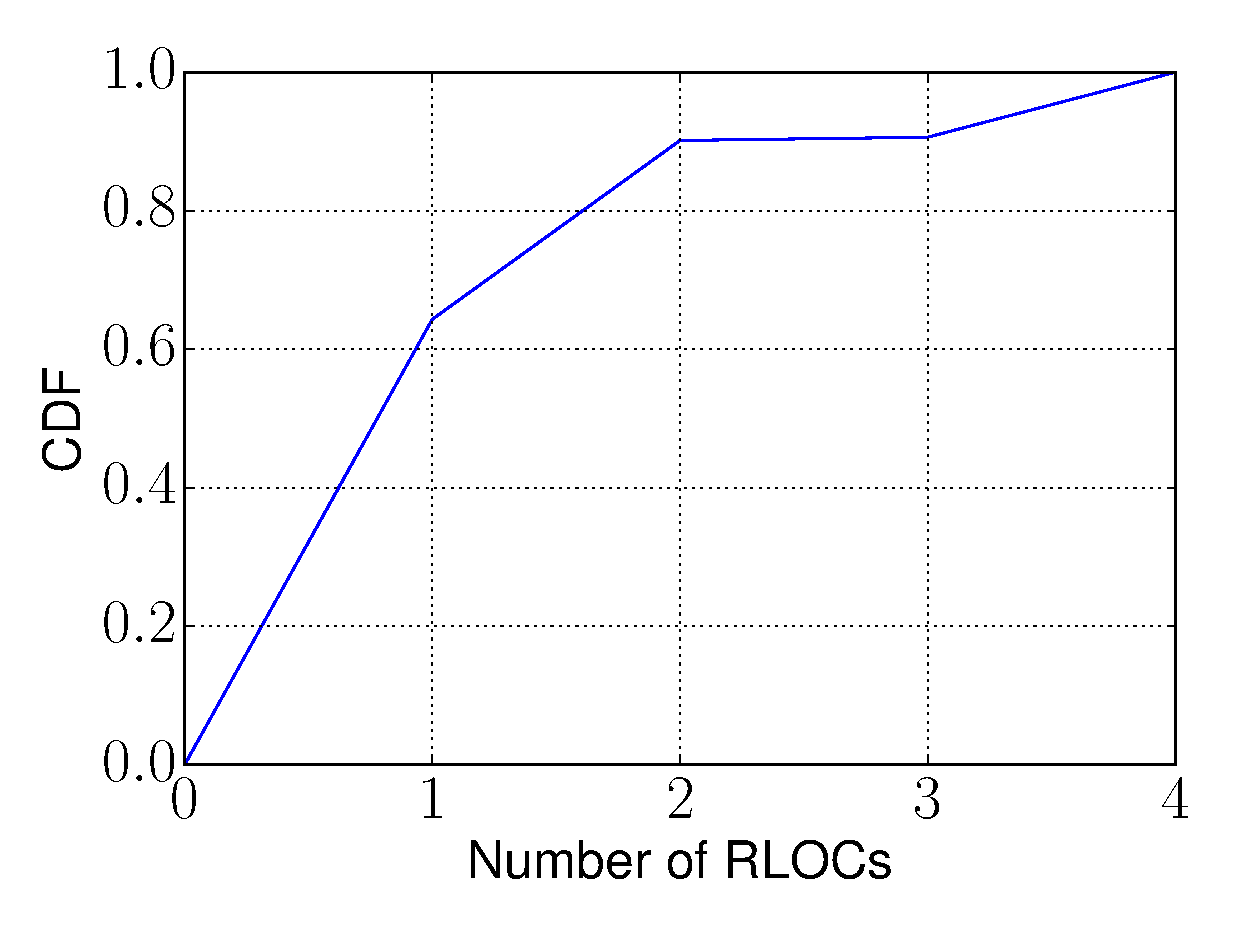
\includegraphics[width=0.8\textwidth]{Pics/CDF_of_RLOCs.eps}
        \caption{CDF of the number of RLOCs}
        \label{CDF_of_RLOCs}
\end{figure}
%-< END FIGURE >--------------------------------------------------------------------

%-< FIGURE >--------------------------------------------------------------------
\begin{figure}[ht]
        \centering
        \includegraphics[width=\linewidth]{Pics/Fig_on_LISPViews.eps}
        \caption{EIDs by Quantity of Associated RLOCs~\cite{lispviews}}
        \label{Fig_on_LISPViews}
\end{figure}
%-< END FIGURE >--------------------------------------------------------------------

The following type of measurement is the distribution of the size of RLOC set,
i.e., how many RLOCs are associated to one EID prefix on average. As
previously observed, the percentage of mappings using two or less RLOCs has
increased between 2010 and $2012$~\cite{lispCCR}. Fig.~\ref{CDF_of_RLOCs}
shows that this trend keeps going on, i.e., more mappings use fewer RLOCs and
the maximum number of RLOC is~4. An interesting point is that although LISP is a
good candidate to support the increasing multi-homing in Internet,
more than 60\% LISP users are not multi-homed and among them the majority
only has 2 RLOCs. Not only the number of RLOCs of each site does significantly
change, but also the RLOCs themselves remains stable. We measured that the
stability reaches 99.8\% for all the dataset, i.e., once an
EID-prefix~--~to~--~RLOCs mapping is decided, it rarely changes. Surprisingly,
we have not found any mobile LISP sites.

All the aforementioned observations are based on the experiment made between
September and October 2016 as described in Sec.~\ref{sec:lispviews_evaluation_meth}.
Later LISP-Views detects that MR2 and MR6 in
Fig.~\ref{median_rtt_per_map-resolver} with very high overall RTTs are down,
and three new other MRs are up. After confirming with the operators of the LISP
Beta Network, these two MRs are indeed definitely down. The change of the
architecture of MRs also proves the accuracy of LISP-Views, while the LISPmon
presents a smooth change in its daily reports, hence hiding these facts. Since
February $2017$ LISP-Views publicly publishes preliminary daily reporting
online~\cite{lispviews}. Development efforts are still ongoing to provide a
complete and production-level website. Fig.~\ref{Fig_on_LISPViews} is a capture
from the website, it is one type of measurement about the number of EID-prefix
quantified by the different size of RLOC set. The shown result is an union of
all MRs during a whole day, to present the most complete mapping information of
the actual LISP deployment. The line on the top indicates the number of LISP
Map-Replies, i.e., the Map-Replies with at least 1 RLOC, which coincides to
the results shown in Fig.~\ref{lispmon_comparison} and is mainly affected by
the EID-prefix with 1 RLOC.  Moreover, the composition of the different sizes
of RLOC set is also rather identical to the one in Fig.~\ref{CDF_of_RLOCs}. The
only difference is that in the previous dataset there is no EID-prefix with 3
RLOCs, while in the latest dataset it appears, but not very stable. In
addition, the line with 3 RLOCs is almost complementary to the line with 4
RLOCs. It is probably caused by one LISP-site that has 4 \acrshort{xtr}s but one being
always down, or the LISP-site having 4 interfaces on a same \acrshort{xtr} among which
one is down. Besides, the number of observed EIDs per day heavily drops two
times in the figure. Since the two valley don't drop to zero, we know that the
problem doesn't come directly from the \acrshort{mds}. Instead, the problem comes from
issues that occurred within the network of the LISP-Views server itself. This
observation highlights the urgent need of distributing VPs.


%-< SECTION >--------------------------------------------------------------------
%\section{LISP-related Discussion and Conclusion}
\section{Conclusion}
\label{sec:lispviews_conclusion}
% \begin{itemize}[noitemsep,topsep=0pt]
%     \item Motivated by the only LISP monitor LISPmon
%     % \begin{itemize}[noitemsep,topsep=0pt]
%     %     \item Queries only from a specific MR on LISP Beta Network
%     %     \item Monitors on one VP
%     %     \item Records just once per day
%     %     \item Publishes results daily
%     % \end{itemize}
%     \item LISP-Views monitors LISP status as user-defined
%     % \begin{itemize}[noitemsep,topsep=0pt]
%     %     \item Queries from all working MRs on both LISP testbeds
%     %     \item Monitors on multiple VPs
%     %     \item Continuously records in a day
%     %     \item Obtains the measurement results on various aspects
%     % \end{itemize}
%     \item LISP-Views provides more information
%     % \begin{itemize}[noitemsep,topsep=0pt]
%     %     \item LISP Map-Replies change a lot even within one day
%     %     \item LISP MRs are not consistent
%     % \end{itemize}
%     \item Further work
%     \begin{itemize}[noitemsep,topsep=0pt]
%         \item Implement a REST API
%         \item Deployment on multiple VPs
%         \item Test IPv6 behavior
%     \end{itemize}
% \end{itemize}

Very little is known about the behavior of LISP in operational environments and it still lacks of troubleshooting tools. Motivated by the only LISP monitor deployed so far, named LISPmon, which records the current LISP status only from a specific MR just once per day, we propose a more dynamic LISP monitoring architecture, namely LISP-Views, so to deepen the understandings on LISP and to ease day-to-day operations and troubleshooting. As LISP-Views aims at being deployed in large scale and dynamic networks, we make a comparison with LISPmon to validate the former one by comparing their behavior during one full month.

It demonstrates that LISP-Views provides more information by discovering more mapping information from all MRs and more complete mapping information of each MR. Furthermore, with our proposed monitoring platform, more mapping system performance metrics such as reliability, latency, and configuration issues can be assessed, which helps for further LISP improvements. LISP-Views is still in the first phase, so the implementation of a REST API, the deployment on multiple VPs and the test of IPv6 behavior are still ongoing and future work. 